\documentclass[dvipsnames,tikz]{standalone}
\usepackage{amsmath}
\usepackage{arevmath}
\usepackage{xcolor}
\usepackage{tikz}
\usetikzlibrary{calc}
\usetikzlibrary{decorations.pathreplacing,calligraphy,3d}


\begin{document}
	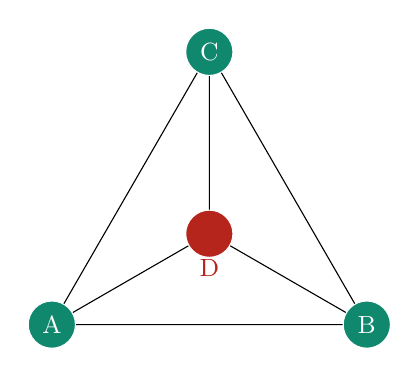
\begin{tikzpicture}[font=\small]
		\draw (0,0) -- (4,0) -- (2,3.464) -- cycle;
		\draw (0,0)-- (2,1.154) -- (2,3.464);
		\draw (2,1.154)-- (4,0);
		
		\draw[white, fill=PineGreen] (0,0) circle (0.3cm) node {A};
		\draw[white, fill=PineGreen] (4,0) circle (0.3cm) node  {B};
		\draw[white, fill=PineGreen] (2,3.464) circle (0.3cm) node {C};
		\draw[white, fill=BrickRed] (2,1.154) circle (0.3cm);
		\draw[white!90!BrickRed] (2,1.154) node {\Large $\skull$};
		\draw[BrickRed] (2,1.154) node [below, yshift=-0.2cm] {D};
	\end{tikzpicture}
\end{document}